\chapter{Monster black holes in compact massive spheroids with intermediate scale discs}
\label{ch:ellic}

This Chapter brings together three ``hot topics'' of today's astrophysical debate, 
that is, over-massive black holes in the $M_{\rm BH} - L_{\rm sph}$ diagram, 
the variety of bulge-to-disc ratios in local early-type galaxies, 
and the evolution of the mass-size relationship from $z=2$ to $z=0$. 
While an overview about the first two topics was given in Sections \ref{sec:monsters} and \ref{sec:photokin}, 
no mention of the mass-size relation was made in Chapter \ref{ch:intro} 
because not immediately related to SMBHs. 
Therefore, a more extensive introduction of this last point is given here. \\ 

It has been claimed that high-redshift passive galaxies were significanly more compact 
than their local counterparts. 
\citet{daddi2005} reported on the observation of seven quiescent early-type galaxies 
at $z=1.4-2.5$ with stellar masses $\gtrsim 10^{11} \rm~M_\odot$ 
and effective radii significantly smaller than those of local couterparts. 
\citet{trujillo2006} analysed ten massive $\approx 5 \times 10^{11} \rm~M_\odot$ galaxies at $z=1.2-1.7$ 
and measured for them sizes a factor of 4 smaller than $z=0$ galaxies with similar stellar masses. 
From this, they concluded that the observed rapid evolution of the structural properties of massive quiescent galaxies 
over the last $\approx 10 \rm~Gyr$ 
cannot be reconciled with a monolithic formation scenario. 
\citet{kriek2008} and \citet{vandokkum2008} found that nearly half of $z \approx 2$ 
massive ($\approx 10^{11} \rm~M_\odot$) galaxies 
have old stellar populations, negligible star formation, and sizes a factor of 5 smaller than 
those of local descendants, 
and silimilar conclusions were reached by several other studies 
(e.g.\citealt{toft2007,trujillo2007,zirm2007,buitrago2008,damjanov2009}). 
While some studies have pointed out that ``progenitor bias''\footnote{``Progenitor bias'' refers to sample confusion 
of the local descendants of high-redhift massive quiescent galaxies. 
While some of the $z=0$ red-sequence galaxies might have had a passive evolution since $z \approx 2$, 
other $z=0$ red-sequence galaxies might descend from $z \approx 2$ star-forming galaxies. } 
(e.g.~\citealt{carollo2014}) might play an important role 
when tracking the evolution of massive quiescent galaxies, 
minor dry mergers have been commonly advocated to explain the size growth of these galaxies 
(e.g.~\citealt{hopkins2009,carrasco2010,cimatti2012,fan2013,de2014}).
However, not enough satellites have been found around massive galaxies 
to support the minor dry mergers scenario 
(e.g.~\citealt{khochfarburkert2006,maller2006,hopkins2009,naab2009,mclure2013}). 
A fascinating solution to the problem was proposed by \citet{graham2013review}, 
who suggested that the high-redshift compact massive spheroids have evolved into the bulges 
of today's massive early-type disc galaxies (see also \citealt{dullograham2013cores} and \citealt{driver2013}). 
This view was confirmed by \citet{gds2015}, 
who used bulge/disc decomposition 
to unveil a large number of previously unnoticed local stellar spheroidal systems 
with the same structural properties, old stellar populations, 
and similar number density as the high-redshift compact massive spheroids. 
\citet{gds2015} advocated the growth of two-dimensional stellar disks around the compact massive spheroids 
to explain the evolution of these objects. \\

The remainder of this chapter comprises the published version of the paper 
``Explaining the reportedly overmassive black holes in early-type galaxies with intermediate-scale discs'' 
by G.~A.~D.~Savorgnan \& A.~W.~Graham,  
as it appears in Volume 457 of \emph{Monthly Notices of the Royal Astronomical Society}. 

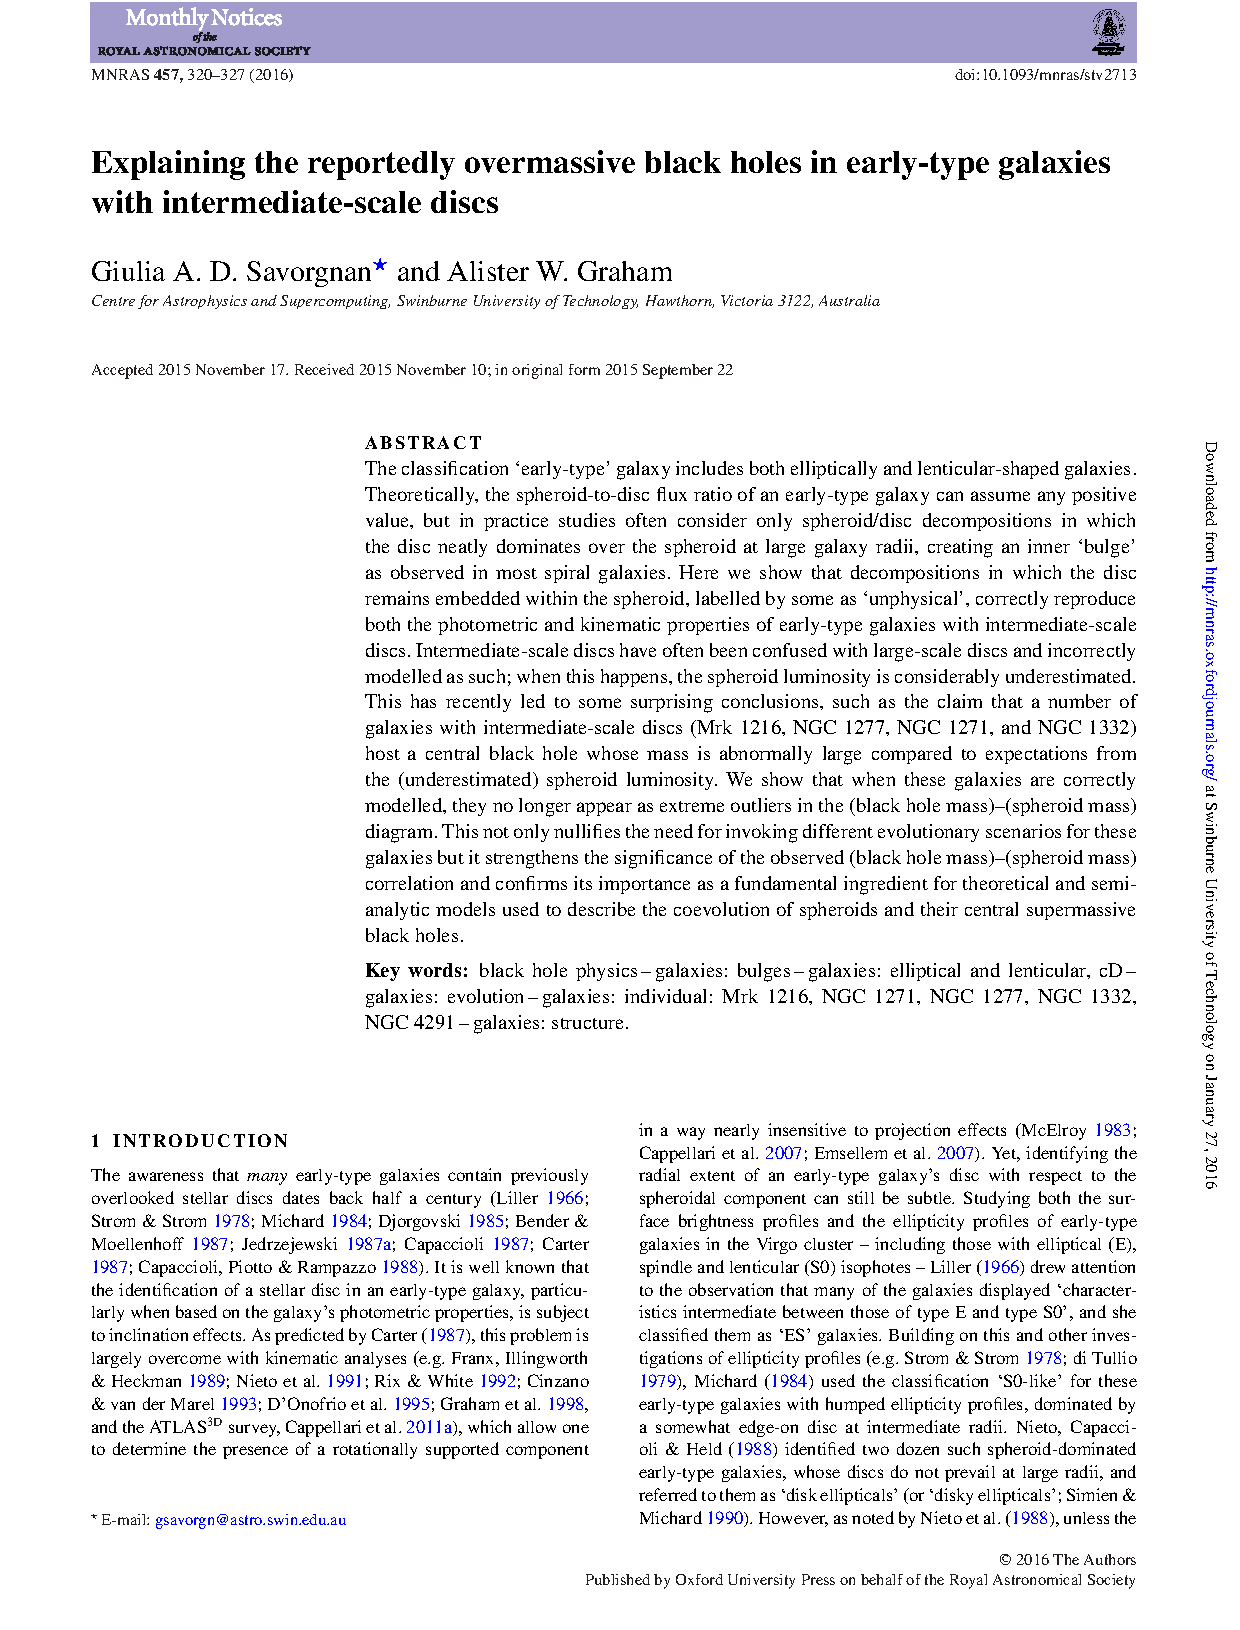
\includepdf[pages={1-8}]{MNRAS2016.pdf}
